\documentclass[10pt,a4paper]{article}\usepackage[]{graphicx}\usepackage[]{color}
%% maxwidth is the original width if it is less than linewidth
%% otherwise use linewidth (to make sure the graphics do not exceed the margin)
\makeatletter
\def\maxwidth{ %
  \ifdim\Gin@nat@width>\linewidth
    \linewidth
  \else
    \Gin@nat@width
  \fi
}
\makeatother

\definecolor{fgcolor}{rgb}{0.345, 0.345, 0.345}
\newcommand{\hlnum}[1]{\textcolor[rgb]{0.686,0.059,0.569}{#1}}%
\newcommand{\hlstr}[1]{\textcolor[rgb]{0.192,0.494,0.8}{#1}}%
\newcommand{\hlcom}[1]{\textcolor[rgb]{0.678,0.584,0.686}{\textit{#1}}}%
\newcommand{\hlopt}[1]{\textcolor[rgb]{0,0,0}{#1}}%
\newcommand{\hlstd}[1]{\textcolor[rgb]{0.345,0.345,0.345}{#1}}%
\newcommand{\hlkwa}[1]{\textcolor[rgb]{0.161,0.373,0.58}{\textbf{#1}}}%
\newcommand{\hlkwb}[1]{\textcolor[rgb]{0.69,0.353,0.396}{#1}}%
\newcommand{\hlkwc}[1]{\textcolor[rgb]{0.333,0.667,0.333}{#1}}%
\newcommand{\hlkwd}[1]{\textcolor[rgb]{0.737,0.353,0.396}{\textbf{#1}}}%
\let\hlipl\hlkwb

\usepackage{framed}
\makeatletter
\newenvironment{kframe}{%
 \def\at@end@of@kframe{}%
 \ifinner\ifhmode%
  \def\at@end@of@kframe{\end{minipage}}%
  \begin{minipage}{\columnwidth}%
 \fi\fi%
 \def\FrameCommand##1{\hskip\@totalleftmargin \hskip-\fboxsep
 \colorbox{shadecolor}{##1}\hskip-\fboxsep
     % There is no \\@totalrightmargin, so:
     \hskip-\linewidth \hskip-\@totalleftmargin \hskip\columnwidth}%
 \MakeFramed {\advance\hsize-\width
   \@totalleftmargin\z@ \linewidth\hsize
   \@setminipage}}%
 {\par\unskip\endMakeFramed%
 \at@end@of@kframe}
\makeatother

\definecolor{shadecolor}{rgb}{.97, .97, .97}
\definecolor{messagecolor}{rgb}{0, 0, 0}
\definecolor{warningcolor}{rgb}{1, 0, 1}
\definecolor{errorcolor}{rgb}{1, 0, 0}
\newenvironment{knitrout}{}{} % an empty environment to be redefined in TeX

\usepackage{alltt}
\usepackage[spanish]{babel}
\usepackage[utf8]{inputenc}
\selectlanguage{spanish}
\title{%
			Examen Final de Modelos Lineales 1 \\
			\large Pontificia Universidad Católica del Perú}
\date{11 de Julio de 2018}
\author{Justo Andrés Manrique Urbina\footnote{e-mail: ja.manrique@pm.me}}
\IfFileExists{upquote.sty}{\usepackage{upquote}}{}
\begin{document}
\maketitle

El presente informe contiene las respuestas del alumno respecto al examen final de Modelos Lineales 1.

\begin{knitrout}\small
\definecolor{shadecolor}{rgb}{0.969, 0.969, 0.969}\color{fgcolor}\begin{kframe}
\begin{alltt}
\hlcom{# Carga de librerías}
\hlkwd{library}\hlstd{(formatR)}
\hlkwd{library}\hlstd{(robustbase)}
\hlkwd{library}\hlstd{(car)}
\hlkwd{library}\hlstd{(stargazer)}
\hlkwd{library}\hlstd{(MASS)}
\hlkwd{library}\hlstd{(agricolae)}
\hlkwd{library}\hlstd{(multcomp)}
\hlkwd{par}\hlstd{(}\hlkwc{mfrow}\hlstd{=}\hlkwd{c}\hlstd{(}\hlnum{2}\hlstd{,}\hlnum{2}\hlstd{))}
\end{alltt}
\end{kframe}
\end{knitrout}

\section{Pregunta 1}

Ver al final del informe.

\section{Pregunta 2}

Ver al final del informe.

\section{Pregunta 3}

Se procede con la carga de los datos en R y renombre de las variables para facilitar el análisis.

\begin{knitrout}\small
\definecolor{shadecolor}{rgb}{0.969, 0.969, 0.969}\color{fgcolor}\begin{kframe}
\begin{alltt}
\hlkwd{rm}\hlstd{(}\hlkwc{list} \hlstd{=} \hlkwd{ls}\hlstd{())}
\hlcom{# Paso 1: Carga de datos}
\hlstd{swiss_1} \hlkwb{<-} \hlkwd{data.frame}\hlstd{(swiss)}

\hlcom{# Paso 2: Renombre de columnas para un análisis más fácil}
\hlkwd{names}\hlstd{(swiss_1)[}\hlnum{1}\hlstd{]} \hlkwb{<-} \hlstr{"Y"}  \hlcom{#Variable Fertility a Y.}
\hlkwd{names}\hlstd{(swiss_1)[}\hlnum{2}\hlstd{]} \hlkwb{<-} \hlstr{"A1"}  \hlcom{#Variable Agriculture a A1.}
\hlkwd{names}\hlstd{(swiss_1)[}\hlnum{3}\hlstd{]} \hlkwb{<-} \hlstr{"A2"}  \hlcom{#Variable Examination a A2.}
\hlkwd{names}\hlstd{(swiss_1)[}\hlnum{4}\hlstd{]} \hlkwb{<-} \hlstr{"A3"}  \hlcom{#Variable Education a A3.}
\hlkwd{names}\hlstd{(swiss_1)[}\hlnum{5}\hlstd{]} \hlkwb{<-} \hlstr{"A4"}  \hlcom{#Variable Catholic a A4.}
\hlkwd{names}\hlstd{(swiss_1)[}\hlnum{6}\hlstd{]} \hlkwb{<-} \hlstr{"A5"}  \hlcom{#Variable Infant Mortality a A5.}
\end{alltt}
\end{kframe}
\end{knitrout}

Posteriormente, se efectúa un análisis descriptivo de los datos. En este se puede apreciar lo siguiente:
\begin{itemize}
	\item La base de datos Swiss se compone de 47 observaciones.
	\item Las variables con mayor variabilidad son las variables A3 y A4, puesto que su desviación estándar es similar a su media (esto daría un coeficiente de variación cercano a 1). Posteriormente, le siguen las variables A2, A1, A5 e Y en ese orden.
\end{itemize}

Ver cuadro a continuación:

\begin{kframe}
\begin{alltt}
\hlkwd{stargazer}\hlstd{(}\hlkwc{title} \hlstd{=}\hlstr{"Análisis descriptivo de datos: Swiss"}\hlstd{,swiss_1,}
\hlkwc{iqr}\hlstd{=}\hlnum{FALSE}\hlstd{,}\hlkwc{flip} \hlstd{=} \hlnum{TRUE}\hlstd{)}
\end{alltt}
\end{kframe}
% Table created by stargazer v.5.2.2 by Marek Hlavac, Harvard University. E-mail: hlavac at fas.harvard.edu
% Date and time: mié., Jul. 11, 2018 - 22:31:28
\begin{table}[!htbp] \centering 
  \caption{Análisis descriptivo de datos: Swiss} 
  \label{} 
\begin{tabular}{@{\extracolsep{5pt}}lcccccc} 
\\[-1.8ex]\hline 
\hline \\[-1.8ex] 
Statistic & Y & A1 & A2 & A3 & A4 & A5 \\ 
\hline \\[-1.8ex] 
N & 47 & 47 & 47 & 47 & 47 & 47 \\ 
Mean & 70.143 & 50.660 & 16.489 & 10.979 & 41.144 & 19.943 \\ 
St. Dev. & 12.492 & 22.711 & 7.978 & 9.615 & 41.705 & 2.913 \\ 
Min & 35.000 & 1 & 3 & 1 & 2.150 & 10.800 \\ 
Pctl(25) & 64.700 & 35.9 & 12 & 6 & 5.195 & 18.150 \\ 
Pctl(75) & 78.450 & 67.7 & 22 & 12 & 93.125 & 21.700 \\ 
Max & 92.500 & 90 & 37 & 53 & 100.000 & 26.600 \\ 
\hline \\[-1.8ex] 
\end{tabular} 
\end{table} 


Con el propósito de evaluar, en primera instancia, posibles indicios de multicolinealidad entre variables, así como identificar las relaciones de las covariables con la variable respuesta, se generó una matriz de correlación con todas las variables contenidas en la base de datos. En esta matriz, se puede apreciar lo siguiente:

\begin{itemize}
	\item La variable A1 tiene una correlación negativa medianamente fuerte con las variables A2 y A3. Por otro lado, dicha variable tiene una correlación positiva mediana con la variable A4.
	\item La variable A2 tiene una correlación positiva medianamente fuerte con la variable A3. Por otro lado, dicha variable tiene una correlación negativa medianamente fuerte con la variable A4.
\end{itemize}

La matriz de correlaciones se puede observar en el Cuadro 2, conforme el siguiente código:

\begin{kframe}
\begin{alltt}
\hlstd{correlation.matrix} \hlkwb{<-} \hlkwd{cor}\hlstd{(swiss_1[,}\hlkwd{c}\hlstd{(}\hlstr{"Y"}\hlstd{,}\hlstr{"A1"}\hlstd{,}\hlstr{"A2"}\hlstd{,}
\hlstr{"A3"}\hlstd{,}\hlstr{"A4"}\hlstd{,}\hlstr{"A5"}\hlstd{)])}
\hlkwd{stargazer}\hlstd{(correlation.matrix,} \hlkwc{title}\hlstd{=}\hlstr{"Matriz de correlaciones"}\hlstd{)}
\end{alltt}
\end{kframe}
% Table created by stargazer v.5.2.2 by Marek Hlavac, Harvard University. E-mail: hlavac at fas.harvard.edu
% Date and time: mié., Jul. 11, 2018 - 22:31:28
\begin{table}[!htbp] \centering 
  \caption{Matriz de correlaciones} 
  \label{} 
\begin{tabular}{@{\extracolsep{5pt}} ccccccc} 
\\[-1.8ex]\hline 
\hline \\[-1.8ex] 
 & Y & A1 & A2 & A3 & A4 & A5 \\ 
\hline \\[-1.8ex] 
Y & $1$ & $0.353$ & $$-$0.646$ & $$-$0.664$ & $0.464$ & $0.417$ \\ 
A1 & $0.353$ & $1$ & $$-$0.687$ & $$-$0.640$ & $0.401$ & $$-$0.061$ \\ 
A2 & $$-$0.646$ & $$-$0.687$ & $1$ & $0.698$ & $$-$0.573$ & $$-$0.114$ \\ 
A3 & $$-$0.664$ & $$-$0.640$ & $0.698$ & $1$ & $$-$0.154$ & $$-$0.099$ \\ 
A4 & $0.464$ & $0.401$ & $$-$0.573$ & $$-$0.154$ & $1$ & $0.175$ \\ 
A5 & $0.417$ & $$-$0.061$ & $$-$0.114$ & $$-$0.099$ & $0.175$ & $1$ \\ 
\hline \\[-1.8ex] 
\end{tabular} 
\end{table} 


Posteriormente, se efectuó una regresión lineal mediante mínimos cuadrados ordinarios, tomando en consideración lo indicado anteriormente. En dicha regresión se observa que:
\begin{itemize}
	\item La variable A2 no es estadísticamente significativa (su p-valor es mayor a 0.05). Por ello, procederemos a descartarla y generar un segundo modelo de regresión lineal.
\end{itemize}

Ambos modelos de regresión se pueden observar en el Cuadro 3 al final de esta sección, conforme el siguiente código:

\begin{kframe}
\begin{alltt}
\hlstd{lm1_swiss} \hlkwb{<-} \hlkwd{lm}\hlstd{(}\hlkwc{formula} \hlstd{= Y} \hlopt{~} \hlstd{A1}\hlopt{+}\hlstd{A2}\hlopt{+}\hlstd{A3}\hlopt{+}\hlstd{A4}\hlopt{+}\hlstd{A5,}
\hlkwc{data}\hlstd{=swiss_1)}
\hlstd{lm2_swiss} \hlkwb{<-} \hlkwd{lm}\hlstd{(}\hlkwc{formula} \hlstd{= Y} \hlopt{~} \hlstd{A1}\hlopt{+}\hlstd{A3}\hlopt{+}\hlstd{A4}\hlopt{+}\hlstd{A5,}
\hlkwc{data}\hlstd{=swiss_1)}
\hlkwd{stargazer}\hlstd{(lm1_swiss,lm2_swiss,} \hlkwc{title}\hlstd{=}\hlstr{"Regresión Lineal"}\hlstd{)}
\end{alltt}
\end{kframe}
% Table created by stargazer v.5.2.2 by Marek Hlavac, Harvard University. E-mail: hlavac at fas.harvard.edu
% Date and time: mié., Jul. 11, 2018 - 22:31:28
\begin{table}[!htbp] \centering 
  \caption{Regresión Lineal} 
  \label{} 
\begin{tabular}{@{\extracolsep{5pt}}lcc} 
\\[-1.8ex]\hline 
\hline \\[-1.8ex] 
 & \multicolumn{2}{c}{\textit{Dependent variable:}} \\ 
\cline{2-3} 
\\[-1.8ex] & \multicolumn{2}{c}{Y} \\ 
\\[-1.8ex] & (1) & (2)\\ 
\hline \\[-1.8ex] 
 A1 & $-$0.172$^{**}$ & $-$0.155$^{**}$ \\ 
  & (0.070) & (0.068) \\ 
  & & \\ 
 A2 & $-$0.258 &  \\ 
  & (0.254) &  \\ 
  & & \\ 
 A3 & $-$0.871$^{***}$ & $-$0.980$^{***}$ \\ 
  & (0.183) & (0.148) \\ 
  & & \\ 
 A4 & 0.104$^{***}$ & 0.125$^{***}$ \\ 
  & (0.035) & (0.029) \\ 
  & & \\ 
 A5 & 1.077$^{***}$ & 1.078$^{***}$ \\ 
  & (0.382) & (0.382) \\ 
  & & \\ 
 Constant & 66.915$^{***}$ & 62.101$^{***}$ \\ 
  & (10.706) & (9.605) \\ 
  & & \\ 
\hline \\[-1.8ex] 
Observations & 47 & 47 \\ 
R$^{2}$ & 0.707 & 0.699 \\ 
Adjusted R$^{2}$ & 0.671 & 0.671 \\ 
Residual Std. Error & 7.165 (df = 41) & 7.168 (df = 42) \\ 
F Statistic & 19.761$^{***}$ (df = 5; 41) & 24.424$^{***}$ (df = 4; 42) \\ 
\hline 
\hline \\[-1.8ex] 
\textit{Note:}  & \multicolumn{2}{r}{$^{*}$p$<$0.1; $^{**}$p$<$0.05; $^{***}$p$<$0.01} \\ 
\end{tabular} 
\end{table} 


\newpage
Una vez definido el modelo a utilizar, se procede a evaluar los supuestos del modelo mediante los siguientes gráficos:

\begin{knitrout}\small
\definecolor{shadecolor}{rgb}{0.969, 0.969, 0.969}\color{fgcolor}\begin{kframe}
\begin{alltt}
\hlkwd{par}\hlstd{(}\hlkwc{mfrow}\hlstd{=}\hlkwd{c}\hlstd{(}\hlnum{2}\hlstd{,}\hlnum{2}\hlstd{))}
\hlkwd{plot}\hlstd{(lm2_swiss,}\hlkwc{main} \hlstd{=} \hlstr{"Diagnóstico de regresión"}\hlstd{)}
\end{alltt}
\end{kframe}
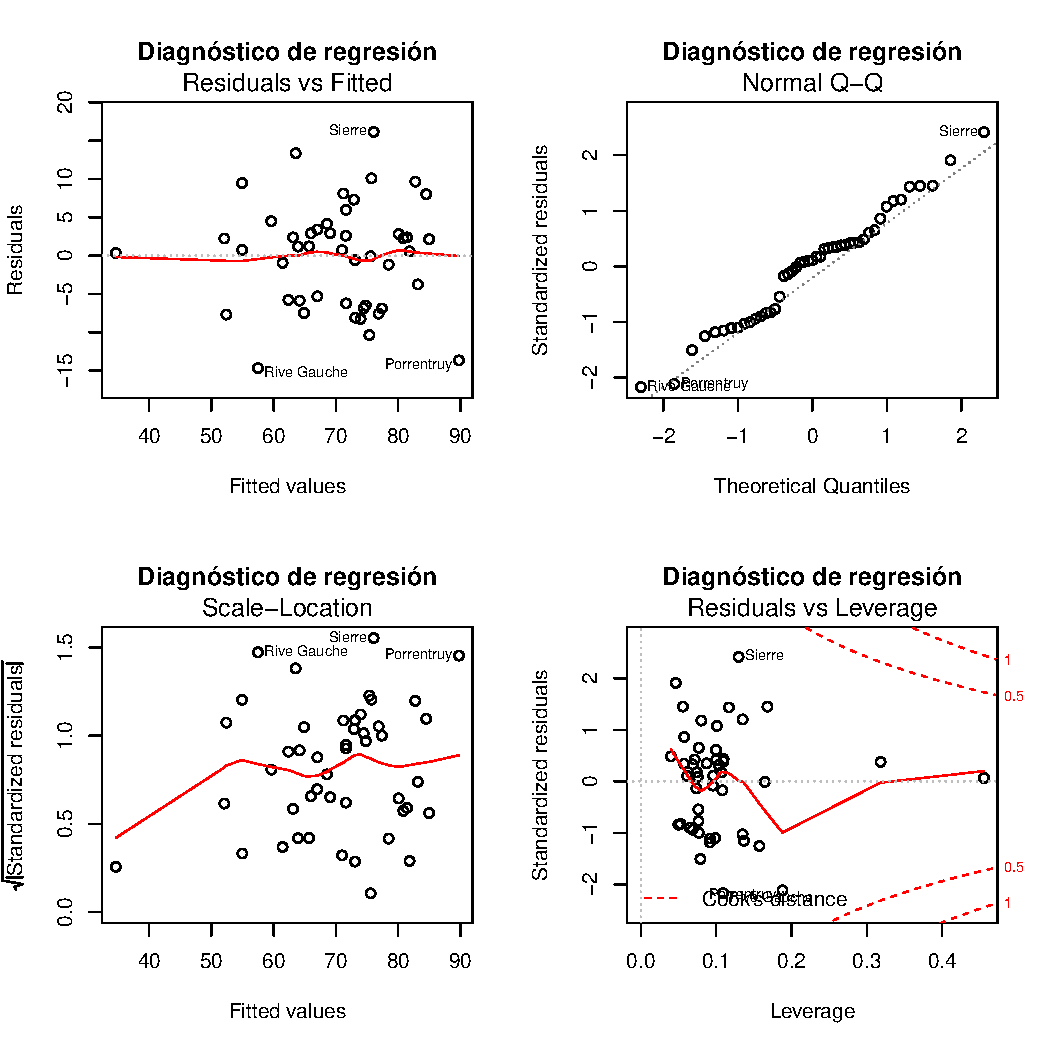
\includegraphics[width=\maxwidth]{figure/evalerrores-1} 

\end{knitrout}

En estos se aprecia lo siguiente:

\begin{itemize}
  \item La gráfica "Residuals vs Fitted" tiene como objetivo identificar si los residuales tienen un comportamiento no lineal. En esta, no se observa una relación no lineal entre los residuales; por lo tanto, se puede inferir no existe una relación no lineal que habría que modelar.
  \item La gráfica "Normal Q-Q" permite identificar si los residuos están normalmente distribuidos. En el caso los residuos no sigan, en general, una línea recta, sería un indicador que los errores no están distribuidos normalmente. En base al cuadro presentado, pueden existir indicios de no-normalidad. Esto se pondrá a prueba a través del test Shapiro-Wilks.
  \item La gráfica "Scale-Location" permite identificar si los errores son homocedásticos o no. En ese sentido, si hubiere algún grado de linealidad en esta gráfica, ello implicaría que los errores no tienen varianza constante por lo que no serían homocedásticos. En base al cuadro presentado, un grado de linealidad en la medida que el valor predicho aumenta; por lo tanto, se podría concluir que los errores son heterocedásticos.
  \item La gráfica "Residuals vs Leverage" permite identificar puntos aberrantes dentro de la base de datos. En base al cuadro presentado, la observación "Sierra" tiene una distancia de Cooks mayor que las otras observaciones. Sin embargo, no supera los umbrales como para tener un impacto significativo.
\end{itemize}

Finalmente, se efectuaron tests estadísticos de homocedasticidad y normalidad de los errores a fin de validar los supuestos de la regresión lineal múltiple bajo mínimos cuadrados ordinarios. Ver resultados a continuación:

\begin{itemize}
  \item Prueba de Normalidad de Errores (Shapiro-Wilks)
    \begin{itemize}
      \item El test de Shapiro-Wilks está orientado a identificar si los errores siguen una distribución normal, a fin de validar los supuestos de la regresión. La hipótesis nula de dicho test es que una determinada muestra proviene de una población normalmente distribuida (Camiz, 2018). Conforme se aprecia en el cuadro posterior, el p-valor del test es mayor a 0.05 por lo que se no serechaza dicha hipótesis nula. Por lo tanto, los residuos seguirían una distribución normal cumpliendo con el supuesto de la regresión.
\begin{knitrout}
\definecolor{shadecolor}{rgb}{0.969, 0.969, 0.969}\color{fgcolor}\begin{kframe}
\begin{verbatim}
## 
## 	Shapiro-Wilk normality test
## 
## data:  lm2_swiss$residuals
## W = 0.97657, p-value = 0.459
\end{verbatim}
\end{kframe}
\end{knitrout}
    \end{itemize}  
  \item Prueba de Homocedasticidad de Errores (Prueba de Breusch-Pagan)
    \begin{itemize}
      \item El test de Breusch-Pagan está orientado a identificar si los errores tienen una varianza homocedástica, a fin de validar los supuestos de la regresión. La hipótesis nula de dicho test es que los errores son homocedásticos (Camiz,2018). Conforme se aprecia en el cuadro posterior, el p-valor del test es menor a 0.05, por lo que no se rechaza la hipótesis nula. Por lo tanto, los residuos tendrían varianza constante cumpliendo con el supuesto de la regresión.
\begin{knitrout}
\definecolor{shadecolor}{rgb}{0.969, 0.969, 0.969}\color{fgcolor}\begin{kframe}
\begin{verbatim}
## Non-constant Variance Score Test 
## Variance formula: ~ fitted.values 
## Chisquare = 0.4687214    Df = 1     p = 0.493576
\end{verbatim}
\end{kframe}
\end{knitrout}
    \end{itemize}
\end{itemize}

\subsection{Corrección de la multicolinealidad}

Con el propósito de corregir la multicolinealidad entre A1, A2 y A3, se propuso crear una variable de interacción entre estas tres, conforme se puede ser en el proceso posterior:

\begin{knitrout}\small
\definecolor{shadecolor}{rgb}{0.969, 0.969, 0.969}\color{fgcolor}\begin{kframe}
\begin{alltt}
\hlstd{lm3_swiss} \hlkwb{<-} \hlkwd{lm}\hlstd{(}\hlkwc{formula} \hlstd{= Y} \hlopt{~} \hlstd{A1}\hlopt{:}\hlstd{A2}\hlopt{:}\hlstd{A3}\hlopt{+}\hlstd{A4}\hlopt{+}\hlstd{A5,}
\hlkwc{data}\hlstd{=swiss_1)}
\hlkwd{summary}\hlstd{(lm3_swiss)}
\end{alltt}
\begin{verbatim}
## 
## Call:
## lm(formula = Y ~ A1:A2:A3 + A4 + A5, data = swiss_1)
## 
## Residuals:
##     Min      1Q  Median      3Q     Max 
## -36.650  -5.673   1.296   4.538  16.498 
## 
## Coefficients:
##               Estimate Std. Error t value Pr(>|t|)    
## (Intercept) 43.8722164  9.9379831   4.415  6.7e-05 ***
## A4           0.0893817  0.0351441   2.543  0.01466 *  
## A5           1.4487495  0.4848625   2.988  0.00463 ** 
## A1:A2:A3    -0.0008858  0.0002666  -3.322  0.00183 ** 
## ---
## Signif. codes:  0 '***' 0.001 '**' 0.01 '*' 0.05 '.' 0.1 ' ' 1
## 
## Residual standard error: 9.428 on 43 degrees of freedom
## Multiple R-squared:  0.4676,	Adjusted R-squared:  0.4304 
## F-statistic: 12.59 on 3 and 43 DF,  p-value: 4.858e-06
\end{verbatim}
\end{kframe}
\end{knitrout}

Se observa que la interacción es estadísticamente significativa	e impacta negativamente en la variable respuesta <<Fertilidad>>. Asimismo, se observa que las variables A4 y A5 tienen un impacto positivo conforme se aprecia en sus coeficientes.
\section{Pregunta 4}

\subsection{Pregunta 4.a)}

Se ajustó un modelo de regresión por mínimos cuadrados ordinarios y se ejecutó la prueba de diagnóstico a través del comando plot() en R. En dicho diagnóstico se prestó atención en la prueba <<Residuals vs. Leverage>> con el propósito de identificar las observaciones atípicas. Se observó que la observación 18 es una observación atípica (supera el umbral de 0.5). Ver gráfico a continuación:

\begin{kframe}
\begin{alltt}
\hlcom{#### Inicio de la pregunta 4 ####}
\hlkwd{rm}\hlstd{(}\hlkwc{list} \hlstd{=} \hlkwd{ls}\hlstd{())}
\hlkwd{data}\hlstd{(coleman)}
\hlkwd{par}\hlstd{(}\hlkwc{mfrow} \hlstd{=} \hlkwd{c}\hlstd{(}\hlnum{2}\hlstd{,} \hlnum{2}\hlstd{))}
\hlstd{fit} \hlkwb{<-} \hlkwd{lm}\hlstd{(}\hlkwc{formula} \hlstd{= Y} \hlopt{~} \hlstd{salaryP} \hlopt{+} \hlstd{fatherWc} \hlopt{+} \hlstd{sstatus} \hlopt{+} \hlstd{teacherSc} \hlopt{+} \hlstd{motherLev,}
    \hlkwc{data} \hlstd{= coleman)}
\hlkwd{plot}\hlstd{(fit)}
\end{alltt}
\end{kframe}
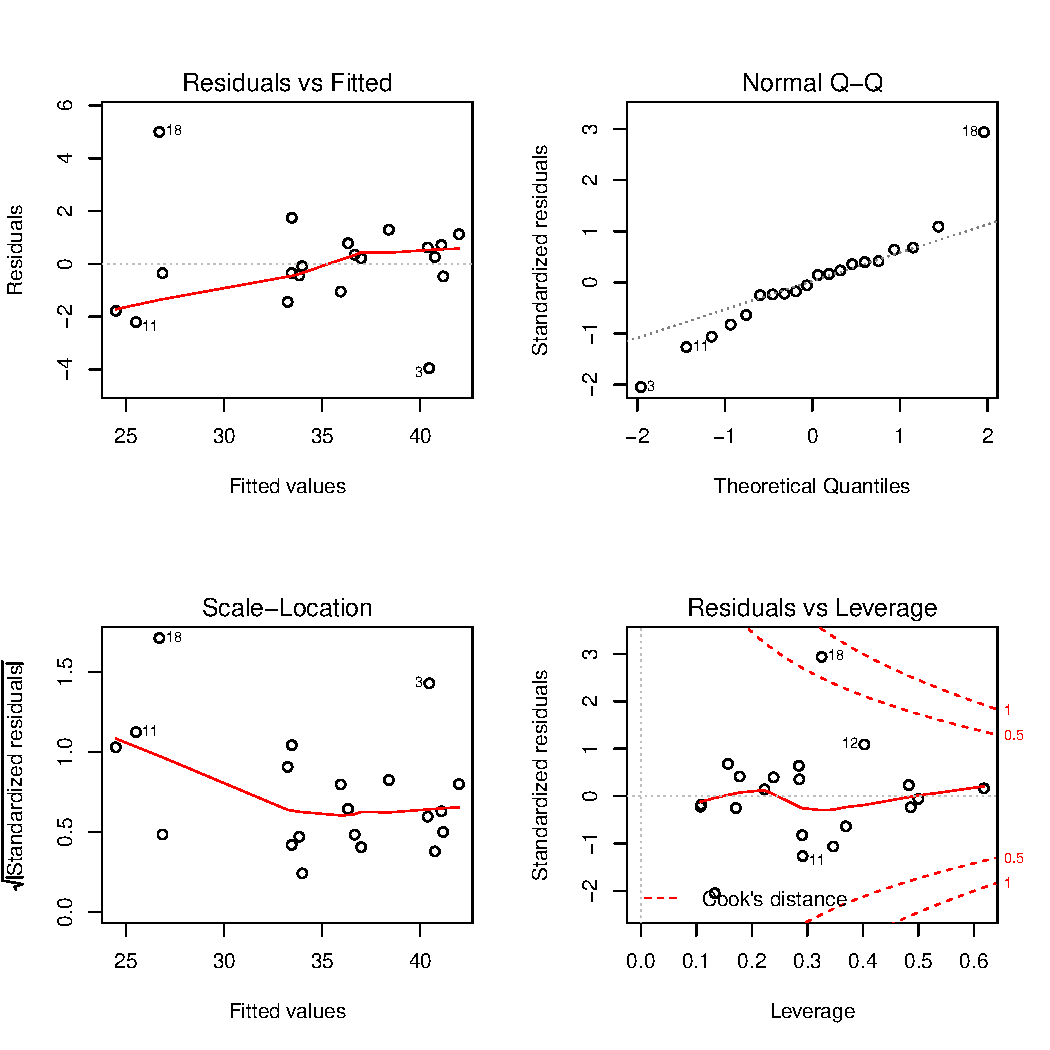
\includegraphics[width=\maxwidth]{figure/Preg_4-1} 


Posteriormente, se generó un nuevo modelo de regresión eliminando dicha observación, y se observa que:
\begin{itemize}
	\item El nuevo modelo de regresión tiene como significativas a todas las variables (exceptuando la variable <<salaryP>>), mientras que el primer modelo de regresión solo mantiene como significativos a las variables <<sstatus>> y <<teacherSC>>.
	\item El nuevo modelo de regresión tiene un R ajustado de 0.949, mientras que el anterior de 0.873.
	\item La variable <<motherLev>> aumentó su coeficiente, de -1.811 a -4.571 con el nuevo modelo de regresión.
	\item La constante del nuevo modelo aumentó 34.287, de 19.949 del modelo anterior.
\end{itemize}

En conclusión, la eliminación de la observación atípica cambió drásticamente la significancia de las variables así como sus coeficientes. Ver código en R dónde se observa la comparación de ambos modelos.

\begin{kframe}
\begin{alltt}
\hlstd{fit_2} \hlkwb{<-} \hlkwd{lm}\hlstd{(}\hlkwc{formula} \hlstd{= Y} \hlopt{~} \hlstd{salaryP} \hlopt{+} \hlstd{fatherWc} \hlopt{+} \hlstd{sstatus} \hlopt{+} \hlstd{teacherSc} \hlopt{+} \hlstd{motherLev,}
    \hlkwc{data} \hlstd{= coleman[}\hlopt{-}\hlkwd{c}\hlstd{(}\hlnum{18}\hlstd{), ])}
\hlkwd{par}\hlstd{(}\hlkwc{mfrow} \hlstd{=} \hlkwd{c}\hlstd{(}\hlnum{2}\hlstd{,} \hlnum{2}\hlstd{))}
\hlkwd{stargazer}\hlstd{(}\hlkwc{title} \hlstd{=} \hlstr{"Regresión Lineal"}\hlstd{, fit, fit_2)}
\end{alltt}
\end{kframe}
% Table created by stargazer v.5.2.2 by Marek Hlavac, Harvard University. E-mail: hlavac at fas.harvard.edu
% Date and time: mié., Jul. 11, 2018 - 22:31:29
\begin{table}[!htbp] \centering 
  \caption{Regresión Lineal} 
  \label{} 
\begin{tabular}{@{\extracolsep{5pt}}lcc} 
\\[-1.8ex]\hline 
\hline \\[-1.8ex] 
 & \multicolumn{2}{c}{\textit{Dependent variable:}} \\ 
\cline{2-3} 
\\[-1.8ex] & \multicolumn{2}{c}{Y} \\ 
\\[-1.8ex] & (1) & (2)\\ 
\hline \\[-1.8ex] 
 salaryP & $-$1.793 & $-$1.617$^{*}$ \\ 
  & (1.233) & (0.794) \\ 
  & & \\ 
 fatherWc & 0.044 & 0.085$^{**}$ \\ 
  & (0.053) & (0.035) \\ 
  & & \\ 
 sstatus & 0.556$^{***}$ & 0.674$^{***}$ \\ 
  & (0.093) & (0.065) \\ 
  & & \\ 
 teacherSc & 1.110$^{**}$ & 1.110$^{***}$ \\ 
  & (0.434) & (0.279) \\ 
  & & \\ 
 motherLev & $-$1.811 & $-$4.571$^{***}$ \\ 
  & (2.027) & (1.437) \\ 
  & & \\ 
 Constant & 19.949 & 34.287$^{***}$ \\ 
  & (13.628) & (9.312) \\ 
  & & \\ 
\hline \\[-1.8ex] 
Observations & 20 & 19 \\ 
R$^{2}$ & 0.906 & 0.963 \\ 
Adjusted R$^{2}$ & 0.873 & 0.949 \\ 
Residual Std. Error & 2.074 (df = 14) & 1.334 (df = 13) \\ 
F Statistic & 27.085$^{***}$ (df = 5; 14) & 68.274$^{***}$ (df = 5; 13) \\ 
\hline 
\hline \\[-1.8ex] 
\textit{Note:}  & \multicolumn{2}{r}{$^{*}$p$<$0.1; $^{**}$p$<$0.05; $^{***}$p$<$0.01} \\ 
\end{tabular} 
\end{table} 

\newpage
\subsection{Pregunta 4.b)}
Se procedió con la generación de la regresión robusta, ver código generado en R:
\begin{kframe}
\begin{alltt}
\hlstd{rob.fit} \hlkwb{<-} \hlkwd{rlm}\hlstd{(}\hlkwc{formula} \hlstd{= Y} \hlopt{~} \hlstd{salaryP} \hlopt{+} \hlstd{fatherWc} \hlopt{+} \hlstd{sstatus} \hlopt{+} \hlstd{teacherSc} \hlopt{+} \hlstd{motherLev,}
    \hlkwc{data} \hlstd{= coleman)}
\hlkwd{stargazer}\hlstd{(}\hlkwc{title} \hlstd{=} \hlstr{"Regresión Lineal"}\hlstd{, fit, fit_2, rob.fit)}
\end{alltt}
\end{kframe}
% Table created by stargazer v.5.2.2 by Marek Hlavac, Harvard University. E-mail: hlavac at fas.harvard.edu
% Date and time: mié., Jul. 11, 2018 - 22:31:29
\begin{table}[!htbp] \centering 
  \caption{Regresión Lineal} 
  \label{} 
\begin{tabular}{@{\extracolsep{5pt}}lccc} 
\\[-1.8ex]\hline 
\hline \\[-1.8ex] 
 & \multicolumn{3}{c}{\textit{Dependent variable:}} \\ 
\cline{2-4} 
\\[-1.8ex] & \multicolumn{3}{c}{Y} \\ 
\\[-1.8ex] & \multicolumn{2}{c}{\textit{OLS}} & \textit{robust} \\ 
 & \multicolumn{2}{c}{\textit{}} & \textit{linear} \\ 
\\[-1.8ex] & (1) & (2) & (3)\\ 
\hline \\[-1.8ex] 
 salaryP & $-$1.793 & $-$1.617$^{*}$ & $-$1.621$^{**}$ \\ 
  & (1.233) & (0.794) & (0.695) \\ 
  & & & \\ 
 fatherWc & 0.044 & 0.085$^{**}$ & 0.075$^{**}$ \\ 
  & (0.053) & (0.035) & (0.030) \\ 
  & & & \\ 
 sstatus & 0.556$^{***}$ & 0.674$^{***}$ & 0.640$^{***}$ \\ 
  & (0.093) & (0.065) & (0.052) \\ 
  & & & \\ 
 teacherSc & 1.110$^{**}$ & 1.110$^{***}$ & 1.156$^{***}$ \\ 
  & (0.434) & (0.279) & (0.244) \\ 
  & & & \\ 
 motherLev & $-$1.811 & $-$4.571$^{***}$ & $-$3.520$^{***}$ \\ 
  & (2.027) & (1.437) & (1.143) \\ 
  & & & \\ 
 Constant & 19.949 & 34.287$^{***}$ & 27.350$^{***}$ \\ 
  & (13.628) & (9.312) & (7.681) \\ 
  & & & \\ 
\hline \\[-1.8ex] 
Observations & 20 & 19 & 20 \\ 
R$^{2}$ & 0.906 & 0.963 &  \\ 
Adjusted R$^{2}$ & 0.873 & 0.949 &  \\ 
Residual Std. Error & 2.074 (df = 14) & 1.334 (df = 13) & 0.746 (df = 14) \\ 
F Statistic & 27.085$^{***}$ (df = 5; 14) & 68.274$^{***}$ (df = 5; 13) &  \\ 
\hline 
\hline \\[-1.8ex] 
\textit{Note:}  & \multicolumn{3}{r}{$^{*}$p$<$0.1; $^{**}$p$<$0.05; $^{***}$p$<$0.01} \\ 
\end{tabular} 
\end{table} 


Se puede observar que:

\begin{itemize}
	\item Las variables contenidas en la regresión robusta, la cual tiene 20 observaciones, son estadísticamente significativas a pesar de la existencia de una variable atípica. Dicho modelo es similar, respecto a la significancia de sus variables, con el modelo lineal bajo mínimos cuadrados ordinarios generado con solo las 19 observaciones (es decir, dónde se elimina la variable atípica).
	\item Respecto a los coeficientes, la regresión robusta tiene mayor similitud con el modelo lineal bajo mínimos cuadrados ordinarios que solo contiene 19 observaciones. Sin embargo, la regresión robusta presenta diferencias por los coeficientes de las variables <<motherLev>> y la constante (-3.520 a -4.571 y 27.350 a 34.287 respectivamente).
\end{itemize}

\section{Pregunta 5}

\subsection{Pregunta 5.a)}
	\begin{itemize}
		\item El factor de bloque consiste en la variable Día, puesto que en esta se prueban cada uno de los silos. Asimismo, es imposible aleatorizar la variable Día.
		\item El factor de tratamiento es compuesto por la variable Silos.
	\end{itemize}
	
\subsection{Pregunta 5.b)}

Las hipótesis estadísticas se encuentran al final del informe.

Ver a continuación el modelo estadístico:
\begin{knitrout}\small
\definecolor{shadecolor}{rgb}{0.969, 0.969, 0.969}\color{fgcolor}\begin{kframe}
\begin{alltt}
\hlkwd{rm}\hlstd{(}\hlkwc{list}\hlstd{=}\hlkwd{ls}\hlstd{())}
\hlstd{silos} \hlkwb{<-} \hlkwd{read.table}\hlstd{(}\hlstr{"D:/Justo Andrés/Dropbox/Maestría en Estadística/2018 - 1/Modelos Lineales 1/Trabajos_/Informe - ML Examen Final/Datos/silos.txt"}\hlstd{,}\hlkwc{header}\hlstd{=}\hlnum{TRUE}\hlstd{)}
\hlstd{mod_silos}\hlkwb{<-}\hlkwd{lm}\hlstd{(temperatura}\hlopt{~}\hlstd{Silo}\hlopt{+}\hlkwd{as.factor}\hlstd{(Dia),silos)}
\hlstd{anova_silos}\hlkwb{<-}\hlkwd{anova}\hlstd{(mod_silos)}
\hlstd{anova_silos}
\end{alltt}
\begin{verbatim}
## Analysis of Variance Table
## 
## Response: temperatura
##                Df Sum Sq Mean Sq F value Pr(>F)
## Silo            4   4.46   1.115  0.6904 0.6092
## as.factor(Dia)  4   9.76   2.440  1.5108 0.2460
## Residuals      16  25.84   1.615
\end{verbatim}
\end{kframe}
\end{knitrout}

Se observa que ambas covariables no son significativas (su p-valor es mayor al umbral de 0.05).

\subsection{Pregunta 5.c)}

Para efectuar el análisis de medias, se utilizó el método de mínimas diferencias. Ver a continuación la ejecución del código:
\begin{knitrout}\small
\definecolor{shadecolor}{rgb}{0.969, 0.969, 0.969}\color{fgcolor}\begin{kframe}
\begin{alltt}
\hlstd{mediat}\hlkwb{<-}\hlkwd{tapply}\hlstd{(silos}\hlopt{$}\hlstd{temperatura,silos}\hlopt{$}\hlstd{Silo,mean)}

\hlstd{difAB} \hlkwb{<-} \hlkwd{abs}\hlstd{(mediat[}\hlnum{1}\hlstd{]}\hlopt{-}\hlstd{mediat[}\hlnum{2}\hlstd{])}
\hlstd{difAC} \hlkwb{<-} \hlkwd{abs}\hlstd{(mediat[}\hlnum{1}\hlstd{]}\hlopt{-}\hlstd{mediat[}\hlnum{3}\hlstd{])}
\hlstd{difAD} \hlkwb{<-} \hlkwd{abs}\hlstd{(mediat[}\hlnum{1}\hlstd{]}\hlopt{-}\hlstd{mediat[}\hlnum{4}\hlstd{])}
\hlstd{difAE} \hlkwb{<-} \hlkwd{abs}\hlstd{(mediat[}\hlnum{1}\hlstd{]}\hlopt{-}\hlstd{mediat[}\hlnum{5}\hlstd{])}
\hlstd{difBC} \hlkwb{<-} \hlkwd{abs}\hlstd{(mediat[}\hlnum{2}\hlstd{]}\hlopt{-}\hlstd{mediat[}\hlnum{3}\hlstd{])}
\hlstd{difBD} \hlkwb{<-} \hlkwd{abs}\hlstd{(mediat[}\hlnum{2}\hlstd{]}\hlopt{-}\hlstd{mediat[}\hlnum{4}\hlstd{])}
\hlstd{difBE} \hlkwb{<-} \hlkwd{abs}\hlstd{(mediat[}\hlnum{2}\hlstd{]}\hlopt{-}\hlstd{mediat[}\hlnum{5}\hlstd{])}
\hlstd{difCD} \hlkwb{<-} \hlkwd{abs}\hlstd{(mediat[}\hlnum{3}\hlstd{]}\hlopt{-}\hlstd{mediat[}\hlnum{4}\hlstd{])}
\hlstd{difCE} \hlkwb{<-} \hlkwd{abs}\hlstd{(mediat[}\hlnum{3}\hlstd{]}\hlopt{-}\hlstd{mediat[}\hlnum{5}\hlstd{])}
\hlstd{difDE} \hlkwb{<-} \hlkwd{abs}\hlstd{(mediat[}\hlnum{4}\hlstd{]}\hlopt{-}\hlstd{mediat[}\hlnum{5}\hlstd{])}

\hlstd{CME} \hlkwb{<-} \hlstd{anova_silos}\hlopt{$}\hlstd{`Mean Sq`[}\hlnum{3}\hlstd{]}
\hlstd{t}\hlkwb{<-} \hlkwd{qt}\hlstd{(}\hlnum{0.975}\hlstd{,anova_silos}\hlopt{$}\hlstd{Df[}\hlnum{3}\hlstd{])}

\hlstd{LSD} \hlkwb{<-} \hlstd{t}\hlopt{*}\hlkwd{sqrt}\hlstd{((}\hlnum{2}\hlopt{*}\hlstd{CME)}\hlopt{/}\hlnum{4}\hlstd{)}
\hlstd{vecdif} \hlkwb{<-} \hlkwd{c}\hlstd{(difAB,difAC,difAD,difAE,difBC,difBD,difBE,difCD,difCE,difDE)}
\hlstd{nombres} \hlkwb{<-} \hlkwd{c}\hlstd{(}\hlstr{"difAB"}\hlstd{,}\hlstr{"difAC"}\hlstd{,}\hlstr{"difAD"}\hlstd{,}\hlstr{"difAE"}\hlstd{,}\hlstr{"difBC"}\hlstd{,}
\hlstr{"difBD"}\hlstd{,}\hlstr{"difBE"}\hlstd{,}\hlstr{"difCD"}\hlstd{,}\hlstr{"difCE"}\hlstd{,}\hlstr{"difDE"}\hlstd{)}

\hlkwa{for}\hlstd{(i} \hlkwa{in} \hlnum{1}\hlopt{:}\hlnum{10}\hlstd{)}
\hlstd{\{}
  \hlkwa{if}\hlstd{(vecdif[i]}\hlopt{>}\hlstd{LSD)}
    \hlkwd{print}\hlstd{(}\hlkwd{paste}\hlstd{(nombres[i],}\hlstr{"Significativa"}\hlstd{))}
  \hlkwa{else}
    \hlkwd{print}\hlstd{(}\hlkwd{paste}\hlstd{(nombres[i],}\hlstr{"No significativa"}\hlstd{))}
\hlstd{\}}
\end{alltt}
\begin{verbatim}
## [1] "difAB No significativa"
## [1] "difAC No significativa"
## [1] "difAD No significativa"
## [1] "difAE No significativa"
## [1] "difBC No significativa"
## [1] "difBD No significativa"
## [1] "difBE No significativa"
## [1] "difCD No significativa"
## [1] "difCE No significativa"
## [1] "difDE No significativa"
\end{verbatim}
\end{kframe}
\end{knitrout}

Se observa que no existen diferencias significativas. Asimismo, se realizó el análisis de diferencias mediante el método Tukey. Ver a continuación el código:

\begin{knitrout}\small
\definecolor{shadecolor}{rgb}{0.969, 0.969, 0.969}\color{fgcolor}\begin{kframe}
\begin{alltt}
\hlstd{amod_1} \hlkwb{<-} \hlkwd{aov}\hlstd{(temperatura} \hlopt{~} \hlstd{Silo} \hlopt{+} \hlkwd{as.factor}\hlstd{(Dia),} \hlkwc{data} \hlstd{= silos)}
\hlstd{compmet_1} \hlkwb{<-} \hlkwd{glht}\hlstd{(amod_1,} \hlkwc{linfct} \hlstd{=} \hlkwd{mcp}\hlstd{(}\hlkwc{Silo} \hlstd{=} \hlstr{"Tukey"}\hlstd{))}
\hlkwd{summary}\hlstd{(compmet_1)}
\end{alltt}
\begin{verbatim}
## 
## 	 Simultaneous Tests for General Linear Hypotheses
## 
## Multiple Comparisons of Means: Tukey Contrasts
## 
## 
## Fit: aov(formula = temperatura ~ Silo + as.factor(Dia), data = silos)
## 
## Linear Hypotheses:
##            Estimate Std. Error t value Pr(>|t|)
## B - A == 0   0.9000     0.8037   1.120    0.794
## C - A == 0   0.1000     0.8037   0.124    1.000
## D - A == 0   1.0000     0.8037   1.244    0.727
## E - A == 0   0.2000     0.8037   0.249    0.999
## C - B == 0  -0.8000     0.8037  -0.995    0.854
## D - B == 0   0.1000     0.8037   0.124    1.000
## E - B == 0  -0.7000     0.8037  -0.871    0.903
## D - C == 0   0.9000     0.8037   1.120    0.794
## E - C == 0   0.1000     0.8037   0.124    1.000
## E - D == 0  -0.8000     0.8037  -0.995    0.854
## (Adjusted p values reported -- single-step method)
\end{verbatim}
\end{kframe}
\end{knitrout}

Se observa que no existen diferencias significativas. 

\section{Pregunta 6}

\subsection{Pregunta 6.a)}

Respuesta al final del Informe.

\subsection{Pregunta 6.b)}

Ver a continuación la ejecución del código R:

\begin{knitrout}\small
\definecolor{shadecolor}{rgb}{0.969, 0.969, 0.969}\color{fgcolor}\begin{kframe}
\begin{alltt}
\hlkwd{rm}\hlstd{(}\hlkwc{list} \hlstd{=} \hlkwd{ls}\hlstd{())}
\hlstd{rdmto} \hlkwb{<-} \hlkwd{read.table}\hlstd{(}\hlstr{"D:/Justo Andrés/Dropbox/Maestría en Estadística/2018 - 1/Modelos Lineales 1/Trabajos_/Informe - ML Examen Final/Datos/rendimiento.txt"}\hlstd{,}
    \hlkwc{header} \hlstd{=} \hlnum{TRUE}\hlstd{)}

\hlstd{mod_rdmto} \hlkwb{<-} \hlkwd{lm}\hlstd{(rendimiento} \hlopt{~} \hlkwd{as.factor}\hlstd{(presion)} \hlopt{+} \hlkwd{as.factor}\hlstd{(temperatura)} \hlopt{+}
    \hlstd{presion} \hlopt{*} \hlstd{temperatura, rdmto)}

\hlstd{anova_rdmto} \hlkwb{<-} \hlkwd{anova}\hlstd{(mod_rdmto)}
\hlstd{anova_rdmto}
\end{alltt}
\begin{verbatim}
## Analysis of Variance Table
## 
## Response: rendimiento
##                        Df  Sum Sq Mean Sq F value    Pr(>F)    
## as.factor(presion)      2 0.76778 0.38389 27.4797 3.313e-05 ***
## as.factor(temperatura)  2 0.30111 0.15056 10.7771  0.002092 ** 
## presion:temperatura     1 0.06125 0.06125  4.3844  0.058171 .  
## Residuals              12 0.16764 0.01397                      
## ---
## Signif. codes:  0 '***' 0.001 '**' 0.01 '*' 0.05 '.' 0.1 ' ' 1
\end{verbatim}
\end{kframe}
\end{knitrout}

Se observa, a través del p-valor, que las variables <<presion>> y <<temperatura>> son significativas. La interacción de ambas variables está muy próxima a la significancia estadística.

\subsection{Pregunta 6.c)}

Ver a continuación la ejecución del código R:

\begin{knitrout}\small
\definecolor{shadecolor}{rgb}{0.969, 0.969, 0.969}\color{fgcolor}\begin{kframe}
\begin{alltt}
\hlkwd{with}\hlstd{(rdmto, (}\hlkwd{interaction.plot}\hlstd{(}\hlkwd{as.factor}\hlstd{(presion),} \hlkwd{as.factor}\hlstd{(temperatura), rendimiento,}
    \hlkwc{type} \hlstd{=} \hlstr{"b"}\hlstd{,} \hlkwc{pch} \hlstd{=} \hlkwd{c}\hlstd{(}\hlnum{18}\hlstd{,} \hlnum{24}\hlstd{,} \hlnum{22}\hlstd{),} \hlkwc{leg.bty} \hlstd{=} \hlstr{"o"}\hlstd{,} \hlkwc{main} \hlstd{=} \hlstr{"Efecto de interacción"}\hlstd{,}
    \hlkwc{xlab} \hlstd{=} \hlstr{"presion"}\hlstd{,} \hlkwc{ylab} \hlstd{=} \hlstr{"rendimiento"}\hlstd{)))}
\end{alltt}
\end{kframe}
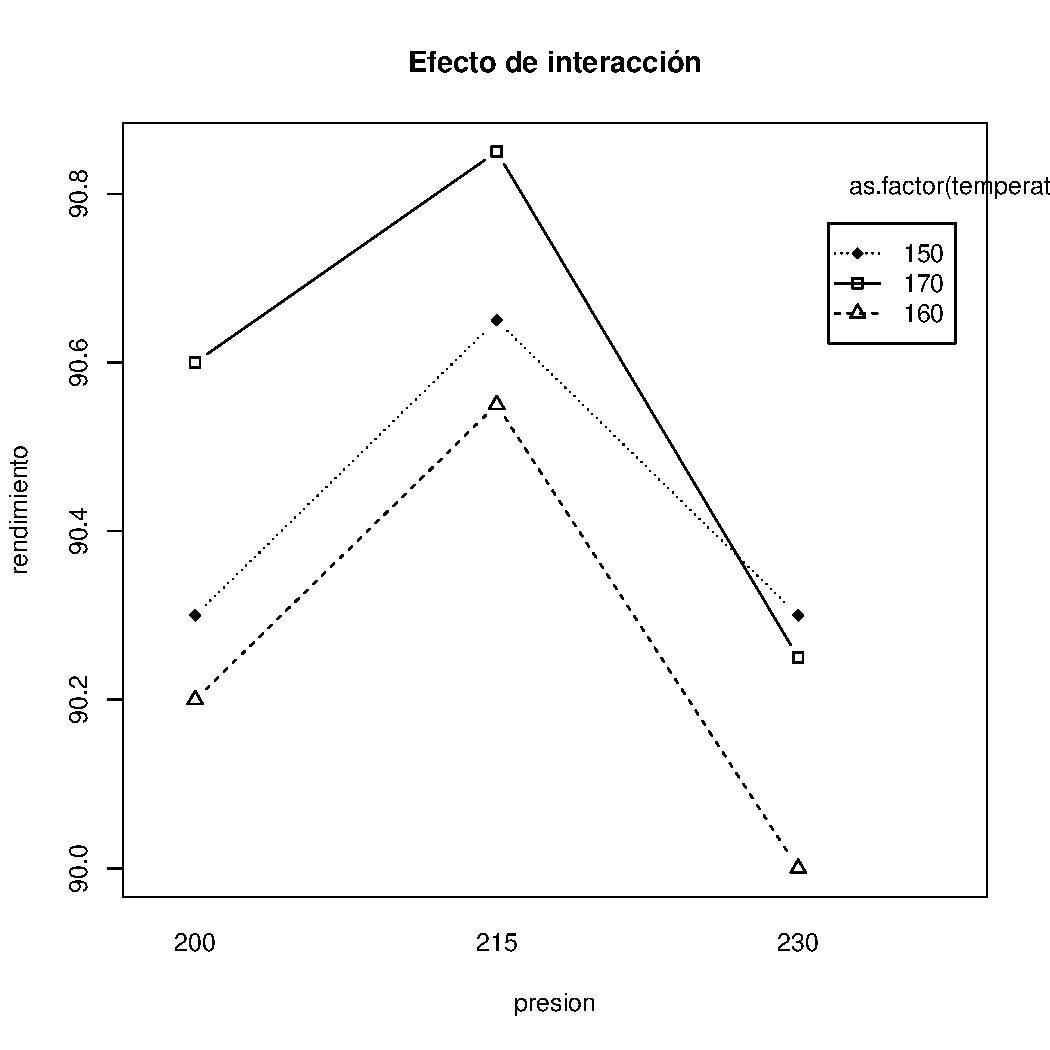
\includegraphics[width=\maxwidth]{figure/preg6_c-1} 
\begin{kframe}\begin{verbatim}
## NULL
\end{verbatim}
\end{kframe}
\end{knitrout}

Se observa que, con el propósito de obtener un mayor rendimiento, la presión debe mantenerse en el valor <<215>> y la temperatura en <<170>>.

\section{Pregunta 7}
\subsection{Pregunta 7.a)}

Ver la generación del gráfico mediante R:
\begin{knitrout}\small
\definecolor{shadecolor}{rgb}{0.969, 0.969, 0.969}\color{fgcolor}\begin{kframe}
\begin{alltt}
\hlkwd{rm}\hlstd{(}\hlkwc{list} \hlstd{=} \hlkwd{ls}\hlstd{())}
\hlstd{fibra} \hlkwb{<-} \hlkwd{read.table}\hlstd{(}\hlstr{"D:/Justo Andrés/Dropbox/Maestría en Estadística/2018 - 1/Modelos Lineales 1/Trabajos_/Informe - ML Examen Final/Datos/fibra.txt"}\hlstd{,}
    \hlkwc{header} \hlstd{=} \hlnum{TRUE}\hlstd{)}
\hlkwd{plot}\hlstd{(fibra}\hlopt{$}\hlstd{resitencia, fibra}\hlopt{$}\hlstd{diametro)}
\end{alltt}
\end{kframe}
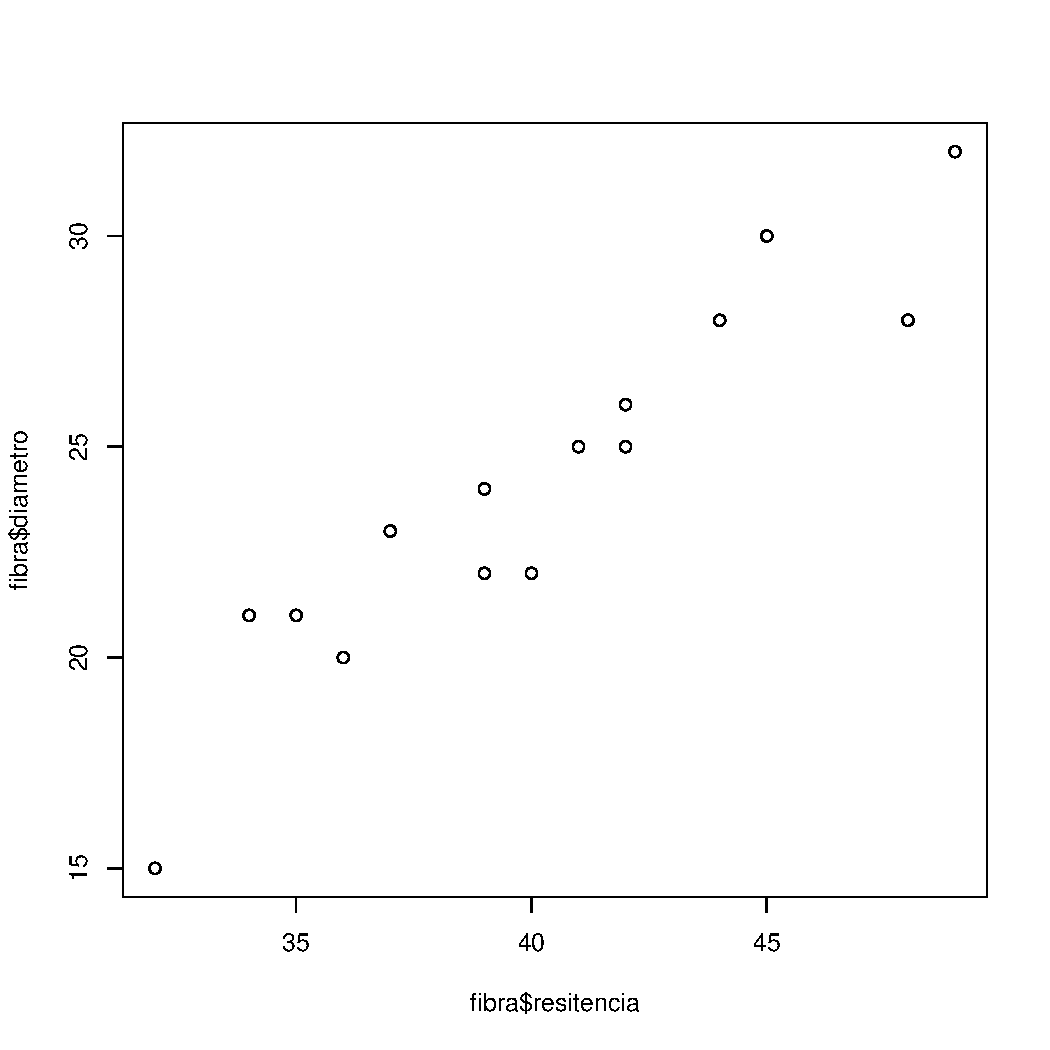
\includegraphics[width=\maxwidth]{figure/preg7_a-1} 
\begin{kframe}\begin{alltt}
\hlkwd{cor}\hlstd{(fibra}\hlopt{$}\hlstd{resitencia, fibra}\hlopt{$}\hlstd{diametro)}
\end{alltt}
\begin{verbatim}
## [1] 0.938542
\end{verbatim}
\end{kframe}
\end{knitrout}

Se observa que existe una relación lineal fuerte entre ambas variables (con un índice de correlación de 0.94). Esto podría deberse a que un mayor diámetro contiene mayor peso, lo cual podría hacerle más resistente.

\subsection{Pregunta 7.b)}
Las hipótesis estadísticas se encuentran al final del informe.

Ver a continuación el código en R respecto al modelo estadístico:

\begin{knitrout}\small
\definecolor{shadecolor}{rgb}{0.969, 0.969, 0.969}\color{fgcolor}\begin{kframe}
\begin{alltt}
\hlstd{mod} \hlkwb{<-} \hlkwd{lm}\hlstd{(resitencia} \hlopt{~} \hlstd{diametro} \hlopt{+} \hlstd{maquina, fibra)}
\hlstd{anova_fibra} \hlkwb{<-} \hlkwd{Anova}\hlstd{(mod,} \hlkwc{type} \hlstd{=} \hlstr{"III"}\hlstd{)}
\hlstd{anova_fibra}
\end{alltt}
\begin{verbatim}
## Anova Table (Type III tests)
## 
## Response: resitencia
##              Sum Sq Df F value    Pr(>F)    
## (Intercept)  87.434  1 34.3664 0.0001089 ***
## diametro    178.014  1 69.9694 4.264e-06 ***
## maquina      13.284  2  2.6106 0.1180839    
## Residuals    27.986 11                      
## ---
## Signif. codes:  0 '***' 0.001 '**' 0.01 '*' 0.05 '.' 0.1 ' ' 1
\end{verbatim}
\end{kframe}
\end{knitrout}

\subsection{Pregunta 7.c)}
Las máquinas, de acuerdo al p-valor obtenido en el ANCOVA anterior, no influye en la resistencia del monofilamento (su p-valor es mayor a 0.05).

\end{document}
